\documentclass[11pt,class=report,crop=false]{standalone}
\usepackage[screen]{../python}


\begin{document}


%====================================================================
\chapitre{Ensemble de Mandelbrot}
%====================================================================

\index{fractale!ensemble de Mandelbrot}
\index{nombre complexe}

\objectifs{Tu vas découvrir un univers encore plus passionnant qu'\emph{Harry Potter} : l'ensemble de Mandelbrot. C'est une fractale, c'est-à-dire que lorsque l'on zoome sur certaines parties de l'ensemble, on retrouve une image similaire à celle de départ. On découvrira aussi les ensembles de Julia.}


\begin{center}
\couleurnb{

\includegraphics[scale=\myscale,scale=0.3]{ecran-mandelbrot-1}
}
{

\includegraphics[scale=\myscale,scale=0.3]{ecran-mandelbrot-1-nb}
}
\end{center}


\objectifs{Voici un zoom, puis un zoom du zoom ! Les points noirs forment l'ensemble de Mandelbrot.}

\begin{center}

\includegraphics[scale=\myscale,scale=0.14]{ecran-mandelbrot-2} \quad
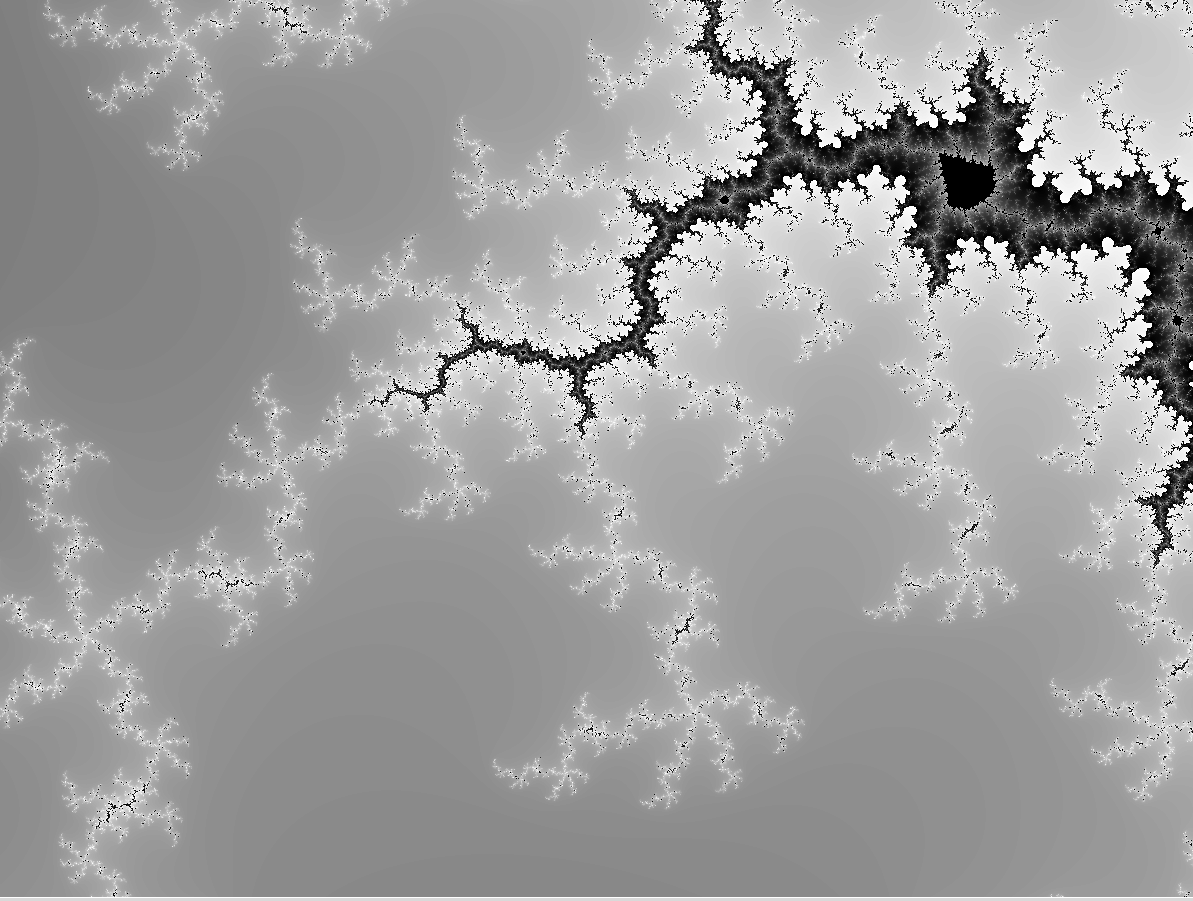
\includegraphics[scale=\myscale,scale=0.14]{ecran-mandelbrot-3}
\end{center}

\objectifs{Cette activité est proposée en deux versions : une avec les nombres complexes (pour ceux qui connaissent) et une version avec les nombres réels.}

%%%%%%%%%%%%%%%%%%%%%%%%%%%%%%%%%%%%%%%%%%%%%%%%%%%%%%%%%%%%%%%%
%%%%%%%%%%%%%%%%%%%%%%%%%%%%%%%%%%%%%%%%%%%%%%%%%%%%%%%%%%%%%%%%

\begin{cours}[L'ensemble de Mandelbrot (avec les nombres complexes)]

\objectifs{Voici la définition de l'ensemble de Mandelbrot pour ceux d'entre vous qui connaissent les nombres complexes.}

On fixe un nombre complexe $c$. On définit une suite de nombres complexes par récurrence :
$$z_0 = 0 \qquad \text{ et pour } n\ge0 \quad z_{n+1} = z_n^2 + c.$$

Si $|z_n|$ ne tend pas vers l'infini (lorsque $n \to +\infty$) alors $c$ est  par définition un point de l'ensemble de Mandelbrot $\mathcal{M}$.

Autrement dit, l'ensemble de Mandelbrot $\mathcal{M}$ est formé de toutes les valeurs $c\in\Cc$ telles que la suite récurrente $(z_n)$ (qui dépend de $c$) reste bornée.
\end{cours}


%%%%%%%%%%%%%%%%%%%%%%%%%%%%%%%%%%%%%%%%%%%%%%%%%%%%%%%%%%%%%%%%
% Activité 1
%%%%%%%%%%%%%%%%%%%%%%%%%%%%%%%%%%%%%%%%%%%%%%%%%%%%%%%%%%%%%%%%

\begin{activite}[Mandelbrot (version complexe)]

\objectifs{Objectifs : préparer le calcul de l'ensemble de Mandelbrot, en utilisant directement les nombres complexes.}

\begin{enumerate}
  \item Programme une fonction (toute simple) \ci{f(z,c)} qui pour $z$ et $c$, des nombres complexes donnés, renvoie $z^2+c$.
  
  \item Programme une fonction \ci{iterer(c)} 
  qui pour un nombre complexe $c$ donné, renvoie le nombre d'itérations qu'il a fallu pour que la suite $(z_n)$ s'échappe \og{}à l'infini\fg{} ; si au bout d'un certain nombre d'itérations la suite ne s'échappe pas, la fonction renvoie $0$.
  

On peut prouver que $(z_n)$ s'échappe vers l'infini dès que l'on trouve $i\ge1$ tel que $|z_i|>2$. On stoppe alors les calculs et on renvoie l'indice $i$.
Si cela n'arrive pas au bout des $100$ premiers termes par exemple, on considère que la suite ne s'échappera jamais et on arrête les calculs (on renvoie $0$), et $c$ est un point de l'ensemble de Mandelbrot.
  
  Voici les détails afin de programmer cette fonction.
  \begin{algorithme}
  \sauteligne 
 \begin{itemize}
   \item
   \begin{itemize}
     \item Entrée : un nombre complexe $c$.
     \item Sortie : le premier indice $i\ge1$ avec $|z_i|>2$, ou $0$ si cela n'arrive pas pour les $\text{MaxIter}$ premiers termes.
   \end{itemize}

  \item Définir la constante $\text{MaxIter}$, par exemple $\text{MaxIter} = 100$.
  
  \item Poser $z=0$ (correspondant à $z_0$).
  
  \item Poser $i=1$.
         
  \item Tant que $|z| \le 2$ et $i < \text{MaxIter}$ :
       \begin{itemize}
         \item Faire \ $z \leftarrow f(z,c)$.
         \item Faire \ $i \leftarrow i+1$.
       \end{itemize}

   \item Une fois la boucle terminée, si $i =\text{MaxIter}$ alors renvoyer $0$, sinon renvoyer $i$.
   
 \end{itemize}  
 \end{algorithme}
  
\end{enumerate} 

\objectifs{Tu peux passer directement à l'activité 3 pour afficher l'ensemble de Mandelbrot.}

\end{activite}



%%%%%%%%%%%%%%%%%%%%%%%%%%%%%%%%%%%%%%%%%%%%%%%%%%%%%%%%%%%%%%%%
%%%%%%%%%%%%%%%%%%%%%%%%%%%%%%%%%%%%%%%%%%%%%%%%%%%%%%%%%%%%%%%%

\begin{cours}[L'ensemble de Mandelbrot (avec les nombres réels)]

\objectifs{Voici la définition de l'ensemble de Mandelbrot pour ceux qui ne connaissent pas encore les nombres complexes.}


On fixe un point du plan $(a,b)$. On définit deux suites réelles par récurrence :
$$x_0= 0 \qquad \text{ et } \qquad y_0 = 0$$
et pour $n\ge0$ :
$$x_{n+1} = x_n^2 - y_n^2 + a \qquad \text{ et} \qquad y_{n+1} = 2 x_n y_n+ b.$$

Si la suite des points $(x_n,y_n)$ ne tend pas vers l'infini (lorsque $n \to +\infty$) alors $(a,b)$ est par définition un point de l'ensemble de Mandelbrot $\mathcal{M}$.

Autrement dit, l'ensemble de Mandelbrot $\mathcal{M}$ est formé de tous les points $(a,b) \in \Rr^2$ tels que la suite des points $(x_n,y_n)$ (qui dépend de $(a,b)$) reste bornée.
\end{cours}




%%%%%%%%%%%%%%%%%%%%%%%%%%%%%%%%%%%%%%%%%%%%%%%%%%%%%%%%%%%%%%%%
% Activité 2
%%%%%%%%%%%%%%%%%%%%%%%%%%%%%%%%%%%%%%%%%%%%%%%%%%%%%%%%%%%%%%%%

\begin{activite}[Mandelbrot (version réelle)]

\objectifs{Objectifs : préparer le calcul de l'ensemble de Mandelbrot, en utilisant uniquement des nombres réels (les nombres complexes restent cachés).}

\begin{enumerate}
  \item Programme une fonction  \ci{f(x,y,a,b)} qui pour $x,y,a,b$, des nombres réels, calcule 
  $$x' = x^2-y^2+a \qquad \text{ et } \qquad y' = 2xy+b$$
  et renvoie les deux nombres réels $x'$ et $y'$.
  
  \item Programme une fonction \ci{iterer(a,b)} 
  qui pour un couple de réel $(a,b)$ donné, renvoie le nombre d'itérations qu'il a fallu pour que la suite $(x_n,y_n)$ s'échappe \og{}à l'infini\fg{} ; si au bout d'un certain nombre d'itérations la suite ne s'échappe pas, la fonction renvoie $0$.
  

On peut prouver que $(x_n,y_n)$ s'échappe vers l'infini dès que l'on trouve $i\ge1$ tel que $x_i^2 + y_i^2 > 4$ . On stoppe alors les calculs et on renvoie l'indice $i$.
Si cela n'arrive pas au bout des $100$ premiers termes par exemple, on considère que la suite ne s'échappera jamais et on arrête les calculs (on renvoie $0$), et $(a,b)$ est un point de l'ensemble de Mandelbrot.
  
  Voici les détails afin de programmer cette fonction.
  \begin{algorithme}
  \sauteligne 
 \begin{itemize}
   \item
   \begin{itemize}
     \item Entrée : un couple de nombres réels $(a,b)$.
     \item Sortie : le premier indice $i\ge1$ avec $x_i^2+y_i^2>4$, ou $0$ si cela n'arrive pas pour les $\text{MaxIter}$ premiers termes.
   \end{itemize}

  \item Définir la constante $\text{MaxIter}$, par exemple $\text{MaxIter} = 100$.
  
  \item Poser $x=0$ et $y=0$ (correspondant à $(x_0,y_0) = (0,0)$).
  
  \item Poser $i=1$.
         
  \item Tant que $x^2+y^2 \le 4$ et $i < \text{MaxIter}$ :
       \begin{itemize}
         \item Faire \ $x,y \leftarrow f(x,y,a,b)$.
         \item Faire \ $i \leftarrow i+1$.
       \end{itemize}

   \item Une fois la boucle terminée, si $i = \text{MaxIter}$ alors renvoyer $0$, sinon renvoyer $i$.
   
 \end{itemize}  
 \end{algorithme}
  
\end{enumerate} 

\objectifs{Dans les activités suivantes tu vas afficher l'ensemble de Mandelbrot.}
\end{activite}




%%%%%%%%%%%%%%%%%%%%%%%%%%%%%%%%%%%%%%%%%%%%%%%%%%%%%%%%%%%%%%%%
% Activité 3
%%%%%%%%%%%%%%%%%%%%%%%%%%%%%%%%%%%%%%%%%%%%%%%%%%%%%%%%%%%%%%%%


\begin{activite}[Préparer l'affichage de l'ensemble de Mandelbrot]

\objectifs{Objectifs : se préparer à afficher l'ensemble de Mandelbrot. Le tout en couleur !}

On utilise le module \ci{tkinter} pour afficher la fractale.

Le code principal sera le suivant (la fonction \ci{mandelbrot()} sera définie dans l'activité suivante) :
\begin{lstlisting}
from tkinter import *
root = Tk()      
canvas = Canvas(root, width=Nx, height=Ny, background="white")
canvas.pack(side=LEFT, padx=5, pady=5)

mandelbrot()

root.mainloop()
\end{lstlisting} 



\begin{enumerate}
  \item  Programme une fonction \ci{afficher_pixel(i,j,couleur)} qui affiche 
  un pixel coloré en position $(i,j)$ d'une fenêtre graphique (qui sera définie après).
 
 Tu peux par exemple tracer un segment à l'aide de \ci{create_line()} de
 $(i,j)$ à $(i+1,j)$.
 
   \item  Programme une fonction \ci{choix_couleur(i)} qui renvoie une couleur en fonction du nombre $i$ (qui correspondra au nombre d'itérations).

\begin{lstlisting}
     if i == 0:
        R,V,B = 0,0,0
    else: 
        R,V,B = 50 + 2*i,0,0
    couleur = '#%02x%02x%02x' % (R, V, B)    
\end{lstlisting}  

  \item Définis des variables \ci{xmin}, \ci{xmax}, \ci{ymin}, \ci{ymax} qui correspondent à la zone de l'ensemble de Mandelbrot à visualiser.
Par exemple pour avoir tout l'ensemble de Mandelbrot on fait :
\begin{lstlisting}
xmin, xmax = -2.2, 1
ymin, ymax = -1.2, 1.2
\end{lstlisting}  



\myfigure{0.7}{
\tikzinput{fig-mandelbrot-1}
}
\begin{center}
\begin{minipage}{0.7\textwidth}
\emph{Le plan de coordonnées $(x,y)$ est représenté sur la figure de gauche ; le grand rectangle correspond à la zone à afficher ; le petit carré est la zone qui sera représentée pas un pixel. Sur la figure de droite c'est l'écran ; les coordonnées sont données par des coordonnées entières $(i,j)$ ; l'écran est composé de pixels (un seul est dessiné), chacun de largeur $1$.}
\end{minipage}
\end{center}

\medskip

  \item Définis deux variables \ci{Nx} et \ci{Ny} qui correspondent à la taille de la fenêtre graphique à afficher.
  Par exemple pour une fenêtre de largeur \ci{Nx}$= 400$ pixels et de hauteur correspondant à la zone à visualiser, faire :
\begin{lstlisting} 
Nx = 400
Ny = round( (ymin-ymax)/(xmin-xmax) * Nx ) 
\end{lstlisting}  
\end{enumerate} 
\end{activite}




%%%%%%%%%%%%%%%%%%%%%%%%%%%%%%%%%%%%%%%%%%%%%%%%%%%%%%%%%%%%%%%%
% Activité 4
%%%%%%%%%%%%%%%%%%%%%%%%%%%%%%%%%%%%%%%%%%%%%%%%%%%%%%%%%%%%%%%%


\begin{activite}[Tracer l'ensemble de Mandelbrot]

\objectifs{Objectifs : dessiner l'ensemble du Mandelbrot ou un zoom.}

\begin{itemize}
  \item Tu as une zone rectangulaire définie par \ci{xmin}, \ci{xmax}, \ci{ymin}, \ci{ymax} qui correspond à la zone de l'ensemble de Mandelbrot à visualiser.

  \item Cette zone s'affichera dans une fenêtre de largeur \ci{Nx} pixels et de hauteur \ci{Ny} pixels.

  \item Définis d'abord deux variables \ci{pasx}, \ci{pasy} qui correspondent à la taille couverte par un pixel selon les formules :
  \mycenterline{\ci{pasx = (xmax-xmin)/Nx} \qquad\qquad \ci{pasy = (ymax-ymin)/Ny}}
 \end{itemize} 
 
 \bigskip
 
  
Programme une fonction \ci{mandelbrot()} qui trace la zone désirée de l'ensemble de Mandelbrot selon les instructions suivantes :

\begin{itemize}
  \item Partir de \ci{a = xmin} et \ci{b = ymin}. 
  \item Pour \ci{i} variant de \ci{0} à \ci{Nx} :
  \begin{itemize}
    \item Pour \ci{j} variant de \ci{0} à \ci{Ny} :
    
    \begin{itemize}
    \item[$\star$] (Version complexe) Poser \ci{c = a + b*1j} (c'est-à-dire $c=a + i b \in \Cc$) et calculer \ci{vitesse = iterer(c)}.
    \item[$\star$] (Version réelle) Calculer \ci{vitesse = iterer(a,b)}. 
  	\item[$\star$] Choisir une  couleur correspondant à la vitesse d'échappement \ci{couleur = choix_couleur(vitesse)}.
  	\item[$\star$] Allumer le pixel correspondant par \ci{afficher_pixel(i,j,couleur)}.
 	\item[$\star$] Faire \ci{b = b + pasy}.
  	\end{itemize}
  	
  	\item Faire \ci{b  = ymin}.
  	\item Faire \ci{a = a + pasx}.
  \end{itemize}
\end{itemize} 


\bigskip 

\objectifs{Le jeu est maintenant double : trouver les plus jolies couleurs possibles (en modifiant la fonction \ci{choix_couleur()}) et surtout chercher des zooms avec les plus belles formes possibles.}

\end{activite}



\bigskip

\objectifs{Les ensembles de Julia se construisent par une méthode proche de celle utilisée pour l'ensemble de Mandelbrot. Cependant les images obtenues sont très différentes et en plus il y a une infinité d'ensembles de Julia possibles.}


\begin{center}
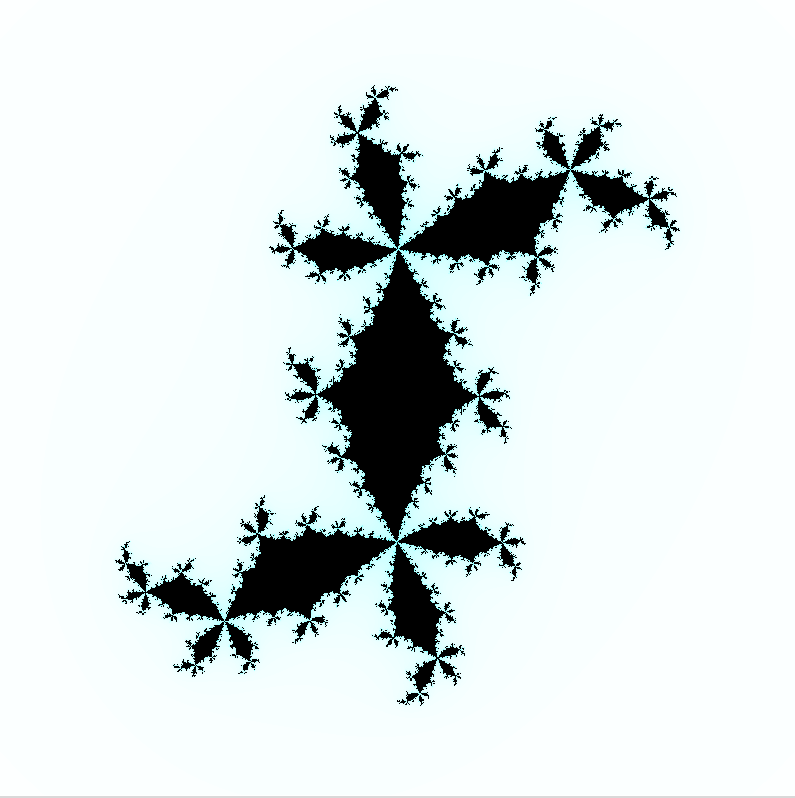
\includegraphics[scale=\myscale,scale=0.20]{ecran-julia-1} \quad

\includegraphics[scale=\myscale,scale=0.20]{ecran-julia-2}
\end{center}

Ci-dessus l'ensemble de Julia avec $c = 0.3+0.55i$ ($a=0.3$, $b=0.55$), appelé le \og{}lapin de Douady\fg{}, avec à droite un zoom.
Ci-dessous l'ensemble de Julia pour $c = -1.31$ (à gauche) et $c=-0.101 + 0.956i$ (à droite).

\begin{center}

\includegraphics[scale=\myscale,scale=0.29]{ecran-julia-3-new} \qquad
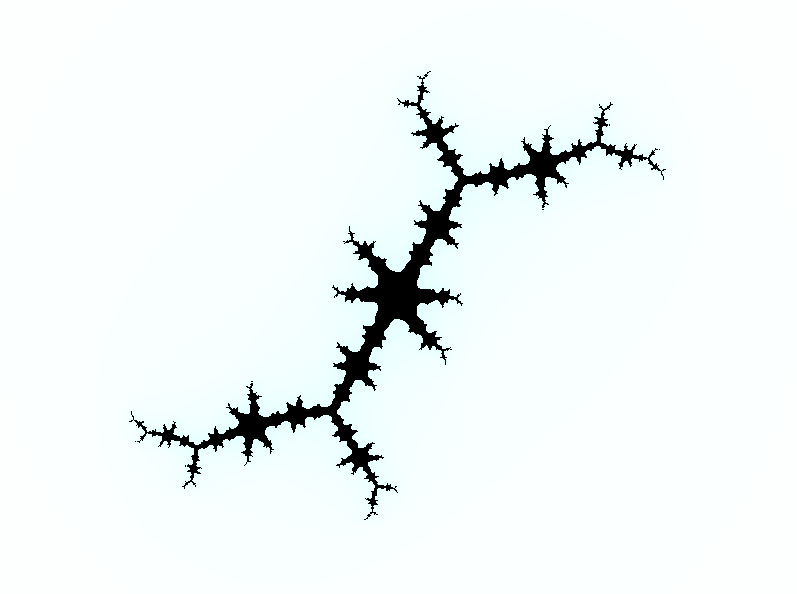
\includegraphics[scale=\myscale,scale=0.20]{ecran-julia-4-new}
\end{center}

%%%%%%%%%%%%%%%%%%%%%%%%%%%%%%%%%%%%%%%%%%%%%%%%%%%%%%%%%%%%%%%%
%%%%%%%%%%%%%%%%%%%%%%%%%%%%%%%%%%%%%%%%%%%%%%%%%%%%%%%%%%%%%%%%

\begin{cours}[Les ensembles de Julia (avec les nombres complexes)]
	
\index{fractale!ensembles de Julia}

\objectifs{Voici la définition des ensembles de Julia pour ceux d'entre vous qui connaissent les nombres complexes.}


On fixe un nombre complexe $c$. On va définir l'ensemble de Julia $\mathcal{J}(c)$ associé à cette valeur.
Pour chaque $z_0 \in \Cc$ on définit une suite de nombres complexes par récurrence pour $n \ge 0$:
$$z_{n+1} = z_n^2 + c$$

Si $|z_n|$ ne tend pas vers l'infini (lorsque $n \to +\infty$) alors $z_0$ est par définition un point de l'ensemble de Julia $\mathcal{J}(c)$.
Cette fois l'ensemble de Julia $\mathcal{J}(c)$ est formé de toutes les valeurs $z_0\in\Cc$ telles que la suite récurrente $(z_n)$ (qui dépend de $z_0$) reste bornée.

La différence avec la définition de l'ensemble de Mandelbrot est qu'ici, le terme $c$ est fixé pour chaque fractale, et c'est le terme initial $z_0$ que l'on fait varier.
\end{cours}


\bigskip

%%%%%%%%%%%%%%%%%%%%%%%%%%%%%%%%%%%%%%%%%%%%%%%%%%%%%%%%%%%%%%%%
% Activité 5
%%%%%%%%%%%%%%%%%%%%%%%%%%%%%%%%%%%%%%%%%%%%%%%%%%%%%%%%%%%%%%%%

\begin{activite}[Julia (version complexe)]

\objectifs{Objectifs : dessiner des ensembles de Julia, 
en utilisant les nombres complexes.}

Il s'agit d'adapter ton programme qui a servi à dessiner l'ensemble de Mandelbrot.

\begin{itemize}
  \item Conserve ta fonction \ci{f(z,c)} qui pour $z$ et $c$, des nombres complexes donnés, renvoie $z^2+c$.
  
  
  \item Adapte la fonction \ci{iterer()} en une fonction \ci{iterer(z0,c)}
  pour tenir compte du terme initial $z_0$.
  
  \item Pour un complexe $c$ fixé, programme une fonction \ci{julia(c)}
  qui affiche l'ensemble de Julia $\mathcal{J}(c)$. C'est presque comme pour l'ensemble de Mandelbrot, mais cette fois lorsque tu fais varier $a,b$ c'est pour définir $z_0 = a + ib$ ; $c$ lui reste fixé.
  
  
\end{itemize}
\end{activite}


\begin{cours}[Les ensembles de Julia (version réelle)]

\objectifs{Voici la définition des ensembles de Julia en utilisant seulement les nombres réels.}


On fixe un couple de réels $(a,b)$. On va définir l'ensemble de Julia $\mathcal{J}(a,b)$ associé à ce couple.
Pour chaque couple $(x_0,y_0) \in \Rr^2$ on définit une suite de nombres réels par récurrence pour $n\ge0$ :
$$x_{n+1} = x_n^2 - y_n^2 + a \qquad \text{ et} \qquad y_{n+1} = 2 x_n y_n + b $$

Si la suite des points $(x_n,y_n)$ ne tend pas vers l'infini (lorsque $n \to +\infty$) alors $(x_0,y_0)$ est par définition un point de l'ensemble de Julia $\mathcal{J}(a,b)$.
Cette fois l'ensemble de Julia $\mathcal{J}(a,b)$ est formé de tous les couples $(x_0,y_0) \in \Rr^2$ tels que la suite $(x_n,y_n)$ (qui dépend de $(x_0,y_0)$) reste bornée.

La différence avec la définition de l'ensemble de Mandelbrot est qu'ici, le couple $(a,b)$ est fixé pour chaque fractale, et c'est le couple initial $(x_0,y_0)$ que l'on fait varier.

\end{cours}



%%%%%%%%%%%%%%%%%%%%%%%%%%%%%%%%%%%%%%%%%%%%%%%%%%%%%%%%%%%%%%%%
% Activité 6
%%%%%%%%%%%%%%%%%%%%%%%%%%%%%%%%%%%%%%%%%%%%%%%%%%%%%%%%%%%%%%%%

\begin{activite}[Julia (version réelle)]

\objectifs{Objectifs : dessiner des ensembles de Julia, 
en utilisant les nombres réels.}

Il s'agit d'adapter ton programme qui a servi à dessiner l'ensemble de Mandelbrot.

\begin{itemize}
  \item Conserve ta fonction \ci{f(x,y,a,b)} qui pour $x,y$ et $a,b$, nombres réels donnés, renvoie les deux réels $x' = x^2-y^2+a$ et $y' = 2xy+b$.
  
  \item Adapte ta fonction \ci{iterer()} en une fonction \ci{iterer(x0,y0,a,b)}
  pour tenir compte des termes initiaux $x_0$ et $y_0$.
  
  \item Pour un couple $(a,b)$ fixé, programme une fonction \ci{julia(a,b)}
  qui affiche l'ensemble de Julia $\mathcal{J}(a,b)$. C'est presque comme pour l'ensemble de Mandelbrot, mais cette fois tu fais varier $x_0$ et $y_0$ à chaque pixel de l'écran ; $a$ et $b$ eux restent fixés.
 
\end{itemize}
\end{activite}

%%%%%%%%%%%%%%%%%%%%%%%%%%%%%%%%%%%%%%%%%%%%%%%%%%%%%%%%%%%%%%%%
%%%%%%%%%%%%%%%%%%%%%%%%%%%%%%%%%%%%%%%%%%%%%%%%%%%%%%%%%%%%%%%%

\begin{cours}[Pour quelques secondes de moins...]
Les calculs pour tracer l'ensemble de Mandelbrot (et ceux de Julia) sont très longs.
Il n'y a pas de solutions immédiates avec \Python{} pour aller plus vite. (Les scripts \Python{} sont interprétés et sont plus longs à exécuter qu'un programme compilé.) 
% (On pourrait utiliser \ci{cython} ou \ci{Numba} pour y remédier.) 

Voici quelques petites astuces pour aller plus vite.
\begin{itemize}
  \item Pour calculer $x^2$ il peut être plus rapide de calculer \ci{x*x} que \ci{x**2}.
  
  \item Il est plus rapide de vérifier $x^2+y^2 > 4$ que $\sqrt{x^2+y^2}>2$.
  
  \item Enfin il est important de ne pas recalculer plusieurs fois la même expression.
  Par exemple à chaque itération, on a besoin de calculer
 $$x' = x^2 - y^2 + a \qquad \text{ et } \qquad y' = 2 x y +  b $$ 
 et de vérifier si 
 $$x^2+y^2 > 4.$$
 Donc on calcule deux fois $x^2$ et deux fois $y^2$.
 Pour éviter cela on peut donc commencer par calculer $x_2= x^2$, $y_2 = y^2$, puis faire les calculs :
  $$x' = x_2 - y_2 + a, \qquad y' = 2 x y +  b \quad \text{ et } \quad x_2+y_2 > 4.$$
  On est donc passé du calcul de $5$ multiplications ($4$ carrés et le produit $xy$) à $3$ multiplications ($2$ carrés et le produit $xy$).
  
  \item Enfin, on peut éviter de calculer des produits de deux nombres différents mais
  uniquement des carrés (en théorie c'est un tout petit peu plus rapide). Il suffit de  remarquer que 
  $$2xy = (x+y)^2 - x^2 - y^2$$
  (il n'y a qu'un nouveau carré à calculer car on a déjà calculé $x^2$ et $y^2$).
  Au total on a donc seulement $3$ carrés à calculer à chaque itération.
\end{itemize}
\end{cours}

\end{document}
